\chapter{Исследовательская часть}

\section{Технические характеристики}

Технические характеристики устройства, на котором выполнялись замеры по времени:

\begin{itemize}
	\item Процессор: Apple M1 Pro \cite{m1}
	\item Оперативная память: 32 ГБайт.
	\item Операционная система: macOS Ventura 13.5.2. \cite{macOS}
\end{itemize}

При замерах времени ноутбук был включен в сеть электропитания и был нагружен только системными приложениями.

\section{Демонстрация работы программы}

На изображении \ref{img:demonstration} представлена иллюстрация работы разработанного программного продукта. 
\clearpage
\begin{figure}[h]
	\centering
	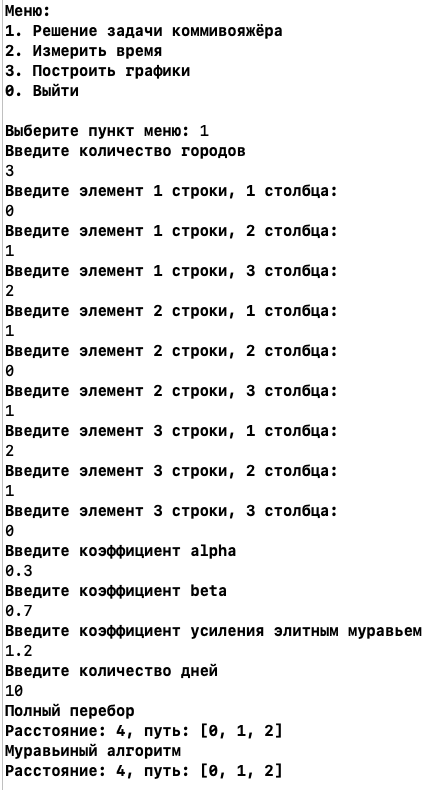
\includegraphics[height=0.6\textheight]{img/example.png}
	\caption{Демонстрация работы программы}
	\label{img:demonstration}
\end{figure}



\clearpage
\section{Анализ временных характеристик}

В данном разделе представлены результаты экспериментов, в которых измерялось время решения задачи коммивояжёра. 
Данные результаты представлены в таблице \ref{tbl:time}.

Таблица \ref{tbl:time} содержит результаты замеров времени выполнения методов решения задачи коммивояжёра: полным перебором и с использованием муравьиного алгоритма.
Замеры проводились для размеров от 1 до 8.
Все замеры проводились 10 раз. 
Брался усредненный результат.

\begin{table}[ht]
	\small
	\begin{center}
		\begin{threeparttable}
		\caption{Результаты замеров времени (массив уже отсортирован)}
		\label{tbl:time}
		\begin{tabular}{|c|c|c|}
			\hline
			& \multicolumn{2}{c|}{\bfseries Время, мс} \\ \cline{2-3}
			\bfseries Размер матрицы & \bfseries Полный перебор & \bfseries Муравьиный алгоритм
			\csvreader{csv/data.csv}{} 
			{\\\hline \csvcoli & \csvcolii & \csvcoliii} \\
			\hline
		\end{tabular}	
		\end{threeparttable}
	\end{center}
\end{table}


На основе данных из таблицы \ref{tbl:time} был построен график (см. рисунок \ref{plt:time}).
\clearpage

\begin{figure}[h]
	\centering
	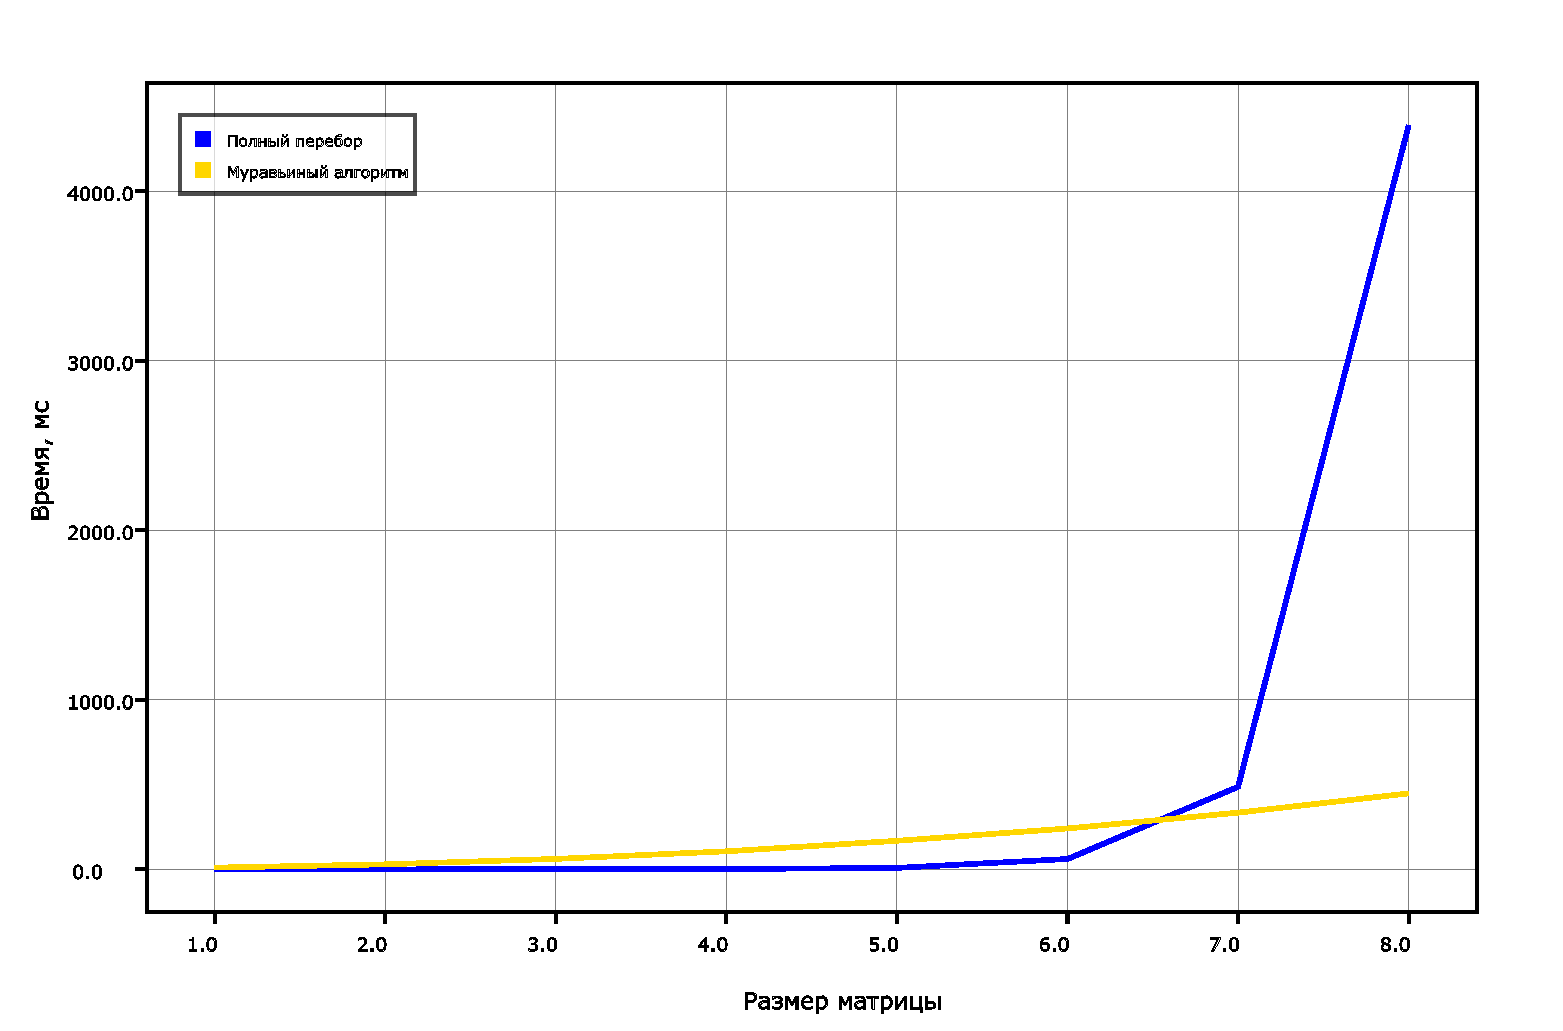
\includegraphics[height=0.4\textheight]{img/graph.pdf}
	\caption{Сравнение времени выполнения методов решения задачи коммивояжёра}
	\label{plt:time}
\end{figure}

\clearpage
\section{Постановка эксперимента}

Цель эксперимента -- найти такие параметры, при которых для выбранного класса данных алгоритм будет возвращать наилучший результат, то есть такой, при котором величина ошибки минимальна.
Таблица значений параметризации будет состоять из следующих значений:

\begin{enumerate}
    \item $\alpha$ -- коэффициент жадности;
    \item $\rho$ -- коэффициент испарения;
    \item $days$ -- количество дней;
    \item $elite$ -- коэффициент усиления элитным муравьем;
    \item $distance$ -- результат, полученный муравьиным алгоритмом при данных параметрах;
    \item $mistake$ -- величина ошибки (разность эталонного результата, полученного методом полного перебора и значения $distance$)
\end{enumerate}

\subsection{Класс данных 1}

Класс данных 1 представляет собой матрицу смежности \ref{eq:matrix1} размером 10x10.
Элементы матрицы - числа от 0 до 100

\begin{equation}
	\label{eq:matrix1}
	M_{1} = \begin{pmatrix}
        0 & 29 & 20 & 21 & 16 & 31 & 100 & 12 & 4 & 31 \\
        29 & 0 & 15 & 35 & 29 & 28 & 40 & 21 & 29 & 41 \\
        20 & 15 & 0 & 18 & 26 & 14 & 43 & 21 & 39 & 40 \\
        21 & 35 & 18 & 0 & 17 & 31 & 38 & 26 & 36 & 27 \\
        16 & 29 & 26 & 17 & 0 & 23 & 45 & 32 & 19 & 21 \\
        31 & 28 & 14 & 31 & 23 & 0 & 27 & 15 & 25 & 37 \\
        100 & 40 & 43 & 38 & 45 & 27 & 0 & 39 & 16 & 18 \\
        12 & 21 & 21 & 26 & 32 & 15 & 39 & 0 & 22 & 23 \\
        4 & 29 & 39 & 36 & 19 & 25 & 16 & 22 & 0 & 26 \\
        31 & 41 & 40 & 27 & 21 & 37 & 18 & 23 & 26 & 0
	\end{pmatrix}
\end{equation}

В таблице \ref{tbl:test1} представлена выборка параметров, при которых муравьиный алгоритм показывает наилучшие результаты.

\begin{table}
	\caption{Результаты параметризации на классе данных 1\label{tbl:test1}}
	\begin{tabular}[c]{|c|c|c|c|c|c|}
        \hline
		$\alpha$ & $\rho$ & $days$ & $elite$ & $distance$ & $mistake$ \\
		\hline
        0.00 & 0.00 & 10.00 & 0.90 & 164.00 & 0.00 \\
        0.00 & 0.00 & 50.00 & 0.00 & 164.00 & 0.00 \\
        0.00 & 0.00 & 50.00 & 0.60 & 164.00 & 0.00 \\
        0.00 & 0.00 & 100.00 & 1.20 & 164.00 & 0.00 \\
        0.00 & 0.10 & 50.00 & 2.00 & 164.00 & 0.00 \\
        0.00 & 0.10 & 100.00 & 0.00 & 164.00 & 0.00 \\
        0.00 & 0.10 & 100.00 & 0.50 & 164.00 & 0.00 \\
        0.00 & 0.10 & 100.00 & 0.80 & 164.00 & 0.00 \\
        0.00 & 0.10 & 100.00 & 1.10 & 164.00 & 0.00 \\
        0.00 & 0.10 & 100.00 & 1.40 & 164.00 & 0.00 \\
        0.00 & 0.10 & 100.00 & 1.50 & 164.00 & 0.00 \\
        0.00 & 0.20 & 50.00 & 0.30 & 164.00 & 0.00 \\
        0.00 & 0.20 & 50.00 & 0.70 & 164.00 & 0.00 \\
        0.00 & 0.30 & 50.00 & 0.50 & 164.00 & 0.00 \\
        0.00 & 0.30 & 50.00 & 0.70 & 164.00 & 0.00 \\
        0.00 & 0.30 & 100.00 & 1.10 & 164.00 & 0.00 \\
        0.00 & 0.30 & 100.00 & 1.20 & 164.00 & 0.00 \\
        0.00 & 0.40 & 100.00 & 0.60 & 164.00 & 0.00 \\
        0.00 & 0.40 & 100.00 & 0.70 & 164.00 & 0.00 \\
        0.00 & 0.50 & 50.00 & 1.40 & 164.00 & 0.00 \\
        0.00 & 0.50 & 50.00 & 2.00 & 164.00 & 0.00 \\
        0.10 & 0.00 & 100.00 & 0.10 & 164.00 & 0.00 \\
        0.10 & 0.10 & 100.00 & 0.20 & 164.00 & 0.00 \\
        0.10 & 0.20 & 100.00 & 0.00 & 164.00 & 0.00 \\
        0.10 & 0.30 & 100.00 & 0.80 & 164.00 & 0.00 \\
        0.10 & 0.40 & 100.00 & 0.60 & 164.00 & 0.00 \\
        0.10 & 0.50 & 50.00 & 0.20 & 164.00 & 0.00 \\
        0.10 & 0.50 & 100.00 & 0.10 & 164.00 & 0.00 \\
        0.10 & 0.60 & 100.00 & 0.20 & 164.00 & 0.00 \\
        0.20 & 0.00 & 50.00 & 1.80 & 164.00 & 0.00 \\
        0.20 & 0.10 & 50.00 & 0.20 & 164.00 & 0.00 \\
        0.20 & 0.10 & 100.00 & 0.20 & 164.00 & 0.00 \\
        0.20 & 0.20 & 50.00 & 0.40 & 164.00 & 0.00 \\
        0.20 & 0.20 & 100.00 & 0.00 & 164.00 & 0.00 \\
        0.20 & 0.30 & 50.00 & 1.30 & 164.00 & 0.00 \\
        0.20 & 0.60 & 10.00 & 1.90 & 164.00 & 0.00 \\
        0.20 & 0.60 & 50.00 & 0.00 & 164.00 & 0.00 \\
        0.30 & 0.00 & 100.00 & 0.50 & 164.00 & 0.00 \\ \hline
    \end{tabular}
\end{table}

\begin{table}
	\caption{Продолжение таблицы \ref{tbl:test1}\label{tbl:test1.1}}
	\begin{tabular}[c]{|c|c|c|c|c|c|}
        \hline
		$\alpha$ & $\rho$ & $days$ & $elite$ & $distance$ & $mistake$ \\
		\hline  
    0.30 & 0.10 & 50.00 & 0.70 & 164.00 & 0.00 \\
        0.30 & 0.30 & 10.00 & 0.40 & 164.00 & 0.00 \\
        0.30 & 0.40 & 50.00 & 0.20 & 164.00 & 0.00 \\
        0.40 & 0.10 & 10.00 & 1.00 & 164.00 & 0.00 \\
        0.40 & 0.20 & 50.00 & 0.10 & 164.00 & 0.00 \\
        0.50 & 0.00 & 100.00 & 0.30 & 164.00 & 0.00 \\
        0.50 & 0.10 & 100.00 & 0.80 & 164.00 & 0.00 \\
        0.50 & 0.40 & 100.00 & 0.90 & 164.00 & 0.00 \\
        0.50 & 0.60 & 10.00 & 1.90 & 164.00 & 0.00 \\
        0.50 & 0.70 & 100.00 & 0.60 & 164.00 & 0.00 \\
        0.60 & 0.10 & 50.00 & 0.50 & 164.00 & 0.00 \\
        0.60 & 0.40 & 100.00 & 0.10 & 164.00 & 0.00 \\
        0.60 & 0.60 & 50.00 & 0.30 & 164.00 & 0.00 \\
        0.60 & 0.70 & 1.00 & 2.00 & 164.00 & 0.00 \\
        0.60 & 0.70 & 100.00 & 0.70 & 164.00 & 0.00 \\
        0.70 & 0.00 & 10.00 & 0.90 & 164.00 & 0.00 \\
        0.70 & 0.10 & 100.00 & 0.60 & 164.00 & 0.00 \\
        0.70 & 0.20 & 50.00 & 1.60 & 164.00 & 0.00 \\
        0.70 & 0.50 & 10.00 & 1.60 & 164.00 & 0.00 \\
        0.70 & 0.70 & 100.00 & 1.70 & 164.00 & 0.00 \\
        0.80 & 0.00 & 100.00 & 1.40 & 164.00 & 0.00 \\
        0.80 & 0.50 & 100.00 & 1.70 & 164.00 & 0.00 \\
        0.80 & 0.70 & 100.00 & 1.70 & 164.00 & 0.00 \\
        0.90 & 0.20 & 100.00 & 1.60 & 164.00 & 0.00 \\
        0.90 & 0.30 & 100.00 & 0.50 & 164.00 & 0.00 \\
        0.90 & 0.30 & 100.00 & 1.90 & 164.00 & 0.00 \\
        0.90 & 0.50 & 100.00 & 0.80 & 164.00 & 0.00 \\
        1.00 & 0.60 & 5.00 & 0.90 & 164.00 & 0.00 \\
        1.00 & 0.70 & 50.00 & 1.70 & 164.00 & 0.00 \\ \hline
    \end{tabular}
\end{table}
\clearpage

\subsection{Класс данных 2}

Класс данных 2 представляет собой матрицу смежности \ref{eq:matrix2} размером 10x10.
Элементы матрицы - числа от 1000 до 10000

\begin{equation}
	\label{eq:matrix2}
	M_{2} = \begin{pmatrix}
        0 & 8200 & 6500 & 7300 & 4800 & 9100 & 10000 & 3200 & 4200 & 8900 \\
        8200 & 0 & 4500 & 9500 & 8100 & 7900 & 9200 & 6600 & 8600 & 9700 \\
        6500 & 4500 & 0 & 6700 & 7800 & 6400 & 9300 & 5200 & 9100 & 9400 \\
        7300 & 9500 & 6700 & 0 & 6200 & 8300 & 9600 & 7400 & 8400 & 9300 \\
        4800 & 8100 & 7800 & 6200 & 0 & 7200 & 9800 & 8500 & 5500 & 5700 \\
        9100 & 7900 & 6400 & 8300 & 7200 & 0 & 7900 & 6300 & 7300 & 8600 \\
        10000 & 9200 & 9300 & 9600 & 9800 & 7900 & 0 & 9700 & 6400 & 6700 \\
        3200 & 6600 & 5200 & 7400 & 8500 & 6300 & 9700 & 0 & 6800 & 7200 \\
        4200 & 8600 & 9100 & 8400 & 5500 & 7300 & 6400 & 6800 & 0 & 7500 \\
        8900 & 9700 & 9400 & 9300 & 5700 & 8600 & 6700 & 7200 & 7500 & 0
	\end{pmatrix}
\end{equation}

В таблице \ref{tbl:test2} представлена выборка параметров, при которых муравьиный алгоритм показывает наилучшие результаты.

\begin{table}
	\caption{Резальтаты параметризации на классе данных 2 \label{tbl:test2}}
	\begin{tabular}[c]{|c|c|c|c|c|c|}
        \hline
		$\alpha$ & $\rho$ & $days$ & $elite$ & $distance$ & $mistake$ \\
		\hline  
        0.00 & 0.00 & 5.00 & 0.70 & 57800.00 & 0.00 \\
        0.00 & 0.00 & 100.00 & 1.50 & 57800.00 & 0.00 \\
        0.00 & 0.10 & 50.00 & 0.90 & 57800.00 & 0.00 \\
        0.00 & 0.20 & 10.00 & 0.10 & 57800.00 & 0.00 \\
        0.00 & 0.40 & 50.00 & 1.70 & 57800.00 & 0.00 \\
        0.00 & 0.40 & 100.00 & 0.60 & 57800.00 & 0.00 \\
        0.00 & 0.40 & 100.00 & 0.70 & 57800.00 & 0.00 \\
        0.00 & 0.50 & 50.00 & 0.70 & 57800.00 & 0.00 \\
        0.00 & 0.50 & 100.00 & 0.20 & 57800.00 & 0.00 \\
        0.00 & 0.50 & 100.00 & 1.00 & 57800.00 & 0.00 \\
        0.00 & 0.50 & 100.00 & 1.10 & 57800.00 & 0.00 \\
        0.00 & 0.60 & 100.00 & 1.50 & 57800.00 & 0.00 \\
        0.10 & 0.10 & 50.00 & 0.90 & 57800.00 & 0.00 \\
        0.10 & 0.30 & 50.00 & 1.70 & 57800.00 & 0.00 \\
        0.10 & 0.40 & 100.00 & 1.20 & 57800.00 & 0.00 \\
        0.10 & 0.40 & 100.00 & 2.00 & 57800.00 & 0.00 \\
        0.10 & 0.50 & 100.00 & 0.70 & 57800.00 & 0.00 \\
        0.10 & 0.60 & 100.00 & 1.80 & 57800.00 & 0.00 \\
        0.10 & 0.70 & 50.00 & 0.50 & 57800.00 & 0.00 \\
        0.10 & 0.70 & 50.00 & 0.90 & 57800.00 & 0.00 \\
        0.10 & 0.70 & 100.00 & 0.90 & 57800.00 & 0.00 \\
        0.10 & 0.70 & 100.00 & 1.60 & 57800.00 & 0.00 \\
        0.10 & 0.70 & 100.00 & 1.70 & 57800.00 & 0.00 \\
        0.20 & 0.10 & 100.00 & 2.00 & 57800.00 & 0.00 \\
        0.20 & 0.20 & 50.00 & 1.60 & 57800.00 & 0.00 \\
        0.20 & 0.40 & 100.00 & 1.50 & 57800.00 & 0.00 \\
        0.20 & 0.50 & 50.00 & 1.80 & 57800.00 & 0.00 \\
        0.20 & 0.50 & 100.00 & 1.00 & 57800.00 & 0.00 \\
        0.20 & 0.60 & 100.00 & 0.50 & 57800.00 & 0.00 \\
        0.30 & 0.20 & 10.00 & 1.60 & 57800.00 & 0.00 \\
        0.30 & 0.30 & 100.00 & 0.40 & 57800.00 & 0.00 \\
        0.30 & 0.50 & 50.00 & 0.10 & 57800.00 & 0.00 \\
        0.40 & 0.00 & 100.00 & 0.40 & 57800.00 & 0.00 \\
        0.40 & 0.10 & 100.00 & 1.30 & 57800.00 & 0.00 \\
        0.40 & 0.20 & 100.00 & 1.00 & 57800.00 & 0.00 \\
        0.40 & 0.20 & 100.00 & 1.60 & 57800.00 & 0.00 \\
        0.40 & 0.30 & 100.00 & 0.00 & 57800.00 & 0.00 \\
        0.40 & 0.30 & 100.00 & 0.10 & 57800.00 & 0.00 \\
        0.40 & 0.50 & 5.00 & 0.70 & 57800.00 & 0.00 \\
        0.40 & 0.60 & 100.00 & 2.00 & 57800.00 & 0.00 \\
        0.40 & 0.70 & 50.00 & 0.00 & 57800.00 & 0.00 \\ \hline
\end{tabular}
\end{table}
\clearpage
\begin{table}
	\caption{Продолжение таблицы \ref{tbl:test2}\label{tbl:test2.1}}
	\begin{tabular}[c]{|c|c|c|c|c|c|}
        \hline
		$\alpha$ & $\rho$ & $days$ & $elite$ & $distance$ & $mistake$ \\
		\hline  
        0.50 & 0.00 & 100.00 & 0.20 & 57800.00 & 0.00 \\
        0.50 & 0.20 & 50.00 & 1.70 & 57800.00 & 0.00 \\
        0.50 & 0.30 & 100.00 & 0.90 & 57800.00 & 0.00 \\
        0.50 & 0.50 & 100.00 & 1.80 & 57800.00 & 0.00 \\
        0.50 & 0.60 & 100.00 & 0.90 & 57800.00 & 0.00 \\
        0.50 & 0.70 & 5.00 & 1.00 & 57800.00 & 0.00 \\
        0.60 & 0.10 & 100.00 & 1.60 & 57800.00 & 0.00 \\
        0.60 & 0.30 & 50.00 & 1.50 & 57800.00 & 0.00 \\
        0.60 & 0.50 & 100.00 & 0.30 & 57800.00 & 0.00 \\
        0.70 & 0.00 & 100.00 & 0.20 & 57800.00 & 0.00 \\
        0.70 & 0.60 & 50.00 & 0.80 & 57800.00 & 0.00 \\
        0.70 & 0.70 & 50.00 & 1.50 & 57800.00 & 0.00 \\
        0.80 & 0.40 & 100.00 & 1.80 & 57800.00 & 0.00 \\
        0.90 & 0.00 & 50.00 & 2.00 & 57800.00 & 0.00 \\
        0.90 & 0.20 & 50.00 & 1.20 & 57800.00 & 0.00 \\
        0.90 & 0.60 & 100.00 & 1.40 & 57800.00 & 0.00 \\
        0.90 & 0.60 & 100.00 & 1.50 & 57800.00 & 0.00 \\
        1.00 & 0.00 & 50.00 & 0.80 & 57800.00 & 0.00 \\
        1.00 & 0.50 & 100.00 & 1.20 & 57800.00 & 0.00 \\ \hline
\end{tabular}
\end{table}
\clearpage
\section{Выводы}
Исходя из полученных результатов, использование муравьиного алгоритма эффективнее по времени использования метода полным перебором при размере входной матрице больше 7.
При этом при размере матрицы равным 7, муравьиный алгоритм эффективнее по времени в 1.5 раза, а при размере равным 8 -- уже в 10 раз.

При проведении экспериментов с классом данных 1, муравьиный алгоритм показывает наилучшие результаты при следующих параметрах:
\begin{enumerate}
    \item $\alpha = 0.0, \rho \in \{0.0, 0.1, 0.3\}$
    \item $\alpha = 0.1, \rho = 0.5$
    \item $\alpha = 0.2, \rho = 0.2$
\end{enumerate}
Для класса данных 2 муравьиный алгоритм показывает наилучшие результаты при параметрах, которые представлены далее:
\begin{enumerate}
    \item $\alpha = 0.0, \rho \in \{0.0, 0.4, 0.5\}$
    \item $\alpha = 0.1, \rho \in \{0.4, 0.7\}$
    \item $\alpha = 0.2, \rho = 0.5$
    \item $\alpha = 0.4, \rho = 0.3$
    \item $\alpha = 0.9, \rho = 0.6$
\end{enumerate}

Именно такие параметры следуюет использовать в муравьином алгоритме на выбранных классах данных.